\documentclass[12pt,twoside]{report}

% PACCHETTI FONDAMENTALI
\usepackage{amsmath,amsfonts,amssymb,amsthm, dsfont, mathtools}
\usepackage{graphicx}
\usepackage[a4paper,outer=2cm,inner=3cm,top=3.3cm,bottom=2.5cm]{geometry}
\usepackage{float} % per il comando [H] per le tabelle
\usepackage{enumerate} % per scegliere i caratteri degli elechi
\usepackage{accents}
\usepackage{esint}
% intestazione pagine
\usepackage{fancyhdr}

% NOMENCLATURA
% indice
\renewcommand*\contentsname{Contents}
% capitoli
\renewcommand{\chaptername}{Chapter}
% appendici
\renewcommand{\appendixname}{Appendices}
% bibliografia
\renewcommand\bibname{Bibliography}
    
% TITOLI
% per mettere i titoli dei capitoli sulla destra e aggiungere una riga di separazione sotto
\usepackage{titlesec} 
\newcommand*{\justifyheading}{\raggedleft}
\titleformat{\chapter}[display]
  {\normalfont\LARGE\bfseries\justifyheading}
  {\chaptertitlename\ \thechapter \vspace*{-0.5cm}}
  {20pt}{\Huge}
  [\vspace*{0.3cm}\hrule height 0.08cm \vspace*{1cm}]

% STUTTURE FONDAMENTALI
% teoremi
\theoremstyle{plain}
\newtheorem{theorem}{Theorem}[section]
% lemmi
\newtheorem{lemma}[theorem]{Lemma}
% teoremi con nomi
\newtheoremstyle{named}{}{}{\itshape}{}{\bfseries}{.}{.5em}{\thmnote{#3} #2}
\theoremstyle{named}
\newtheorem{namedtheorem}[theorem]{Theorem}
% ipotesi
\newenvironment{ipotesi}%
{\quad\left|\quad\def\arraystretch{1.2}\begin{array}{@{}l@{}}}%
{\end{array}\right.}
% tesi
\newcommand{\tesi}[1]{\quad\left|\quad{#1}\right.}
% unico comando per ipotesi e tesi
\newcommand{\hpth}[2]
{
\begin{flalign*}
\quad\quad
\text{Hypothesis}
&\begin{ipotesi}
#1
\end{ipotesi}&&\\
\quad\quad
\text{Thesis}
&\tesi{#2}&&
\end{flalign*}
}
% quando ci sono 2 tesi distinte
\newcommand{\hpthth}[3]
{
\begin{flalign*}
\quad\quad
\text{Hypothesis}
&\begin{ipotesi} 
#1
\end{ipotesi}&&\\
\quad\quad
\text{Thesis 1}
&\tesi{#2}&&\\
\quad\quad
\text{Thesis 2}
&\tesi{#3}&&
\end{flalign*}
}
% dimostrazioni
\renewcommand*{\proofname}{\bf{Proof:}}
\renewcommand\qedsymbol{\textsc{qed}}
% definizioni
\theoremstyle{definition}
\newtheorem{definition}{Definition}[section]
% esempi
\newtheorem{example}{Example}
% osservazioni
\theoremstyle{remark}
\newtheorem*{remark}{Remark}

% NOTAZIONE
% sistemi
\newenvironment{system}%
{\left\lbrace\begin{array}{@{}l@{}}}%
{\end{array}\right.}
% parte intera
\newcommand{\interior}[1]{\accentset{\circ}{#1}}
% norma
\newcommand\norm[1]{\left\lVert#1\right\rVert}
% absolute value
\newcommand\abs[1]{\left|#1\right|}

% PAGINA BIANCA
\usepackage{afterpage}
\newcommand\blankpage{%
    \null
    \thispagestyle{empty}%
    \newpage}

% ALTRI
% indentazione del testo a 0
\parindent 0px
% numerazione in align*
\newcommand\numberthis{\addtocounter{equation}{1}\tag{\theequation}}
% citazione
\usepackage{epigraph}
% immagini
\usepackage{wrapfig}




\begin{document}
% non contare la pagina del titolo
\pagenumbering{gobble}

% titolo
\thispagestyle{empty}

\mdseries{

\vspace*{-1.5cm}
\begin{center}
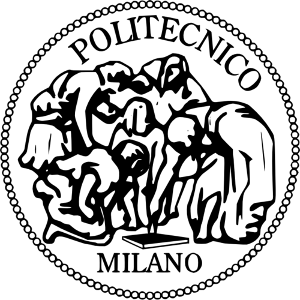
\includegraphics[width=5cm]{logo.png}

\vspace*{0.6cm}
{\LARGE\textsc{Politecnico di Milano}}\\
\rule{8.5cm}{1pt}

\vspace*{0.5cm}
{\large
Corso di Laurea Triennale in \textsc{Ingegneria Matematica}\\
Scuola di \textsc{Ingegneria Industriale e dell'Informazione}\\}

\vspace*{2.5cm} 
{\LARGE\textmd{\textbf{
The Cauchy-Kowalevski Theorem \\ 
\vspace*{2mm} 
and Its Consequences 
}}}
\vspace*{2.5cm} 

{\large
Thesis by
\vspace*{0.3cm}\\
Alessandro Pedone\\
Student ID 981105

\vspace*{1.75cm} 
Advisor:
\vspace*{0.3cm}
\\Prof. Maurizio Grasselli

\vfill
\rule{7.75cm}{1pt}

Graduation Session September 2024\\
\vspace*{1mm}
Academic Year 2023/2024}
\end{center} 
\clearpage
}
\blankpage


% conta con i numeri romani 
\pagenumbering{roman}

% citazione
\setlength\epigraphwidth{8cm}
\setlength\epigraphrule{0pt}
\vspace*{\fill}
\epigraph{\textit{All his life -- he had difficulty saying this, as he admitted, being always wary of too much enthusiasm -- all his life he had been waiting for such a student to come into this room. 
\\A student who would challenge him completely, who was not only capable of following the strivings of his own mind but perhaps of flying beyond them.}}{--- \textup{Alice Munro}, \textit{Too Much Happiness}}
\vspace*{\fill}

\newpage
\blankpage
\chapter*{Abstract}
\addcontentsline{toc}{chapter}{Abstract}

Sofya Kowalevski, la prima donna ad conseguire un dottorato in matematica in Europa, nel 1874 dava la luce alla dimostrazione del teorema di Cauchy-Kowalevski (TCK), il primo risultato generale per l'esistenza di soluzioni locali analitiche per equazioni differenziali alle derivate parziali (EDP) con dati di Cauchy.

\vspace{6mm}
La tesi mira a presentare questa pietra miliare della matematica esaltandone la profondità del dettaglio, le conseguenze e anche la semplicità delle idee che ha permesso di far emergere. A questo scopo sono ricorrenti i richiami di nozioni e risultati fondamentali ad affrontare il discorso e, inoltre, vengono trattate tutte le forme principali in cui è possibile enunciare il TCK.

\vspace{6mm}
A completamento sono presenti anche una sezione dedicata a tre esempi storicamente cruciali alla comprensione delle EDP e un'altra dedicata, invece, alle due sue fondamentali applicazioni: il teorema di Holmgren e il teorema di Cartan-Kähler.

\vspace{6mm}
\textbf{Parole chiave:} EDP, caratteristiche, analiticità/olomorfia, serie di potenze, metodo dei maggioranti, teoremi di Cauchy-Kowalevski, Holmgren e Cartan-Kähler

\newpage
\blankpage
%indice
\tableofcontents

% ricomincia a contare con i numeri arabi
\newpage
\blankpage
\pagenumbering{arabic}

% rimuovi i numeri a piè di pagina
\makeatletter
\let\ps@plain\ps@empty
\makeatother

% inserisci le intestazioni per i capitoli
\pagestyle{fancy}
\renewcommand{\chaptermark}[1]{\markboth{\textit{\thechapter.\ #1}}{}}
\renewcommand{\sectionmark}[1]{\markright{\textit{\thesection.\ #1}}}
\fancyhead{} % cancella tutti i campi
\fancyhead[RO,LE]{\bfseries \thepage}
\renewcommand{\headrulewidth}{0.4pt}
\cfoot{}
\fancyhead[LO]{\rightmark}
\fancyhead[RE]{\leftmark}
\setlength{\headheight}{18pt}

\chapter{Introduction}

\section{Who Was Kowalevski?}
\begin{wrapfigure}{i}{0.25\textwidth}
\centering
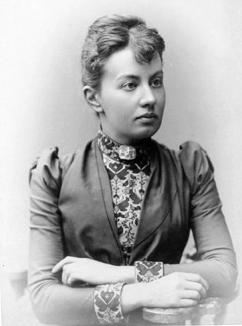
\includegraphics[width=0.25\textwidth]{kovalevskaya_8}
\end{wrapfigure}

Sofya Vasilyevna Kovalevskaya (1850-1891) was a Russian mathematician. For various reasons, including the theorem at the center of this discussion, she remains one of the most significant female figures in the history of this discipline.

First of all, it is important to note that from here on, we will often refer to her by the name she used to sign her publications, namely Kowalevski.

To leave Russia, she had to enter into a marriage of convenience; she married a man with whom she did not have any real emotional relationship and from whom she was often geographically distant. This allowed her to continue her studies in Germany, where she met Karl Weierstrass, one of the most influential mathematicians of his time. After their initial meeting in the professor's study, their relationship continued to develop thanks to Kowalevski's evident mathematical talents, which Weierstrass could not help but nurture. In fact, he continued to give her private lessons, eventually supervising her research work.

Regarding Kowalevski's political ideas, we can historically assert her closeness to feminist movements and socialist and radical ideas, which can be traced back to her family background and the insights she gained from her experiences in the states of modern Europe. It is certainly noteworthy that she received several copies of radical magazines of that time from her sister Anna, which discussed the so-called ancient nihilism\footnote{For ancient nihilists, science, rather than religion and superstition, appeared to be the most effective means of helping the population, thus representing truth and progress.}.

However, our focus is not on her political, social, and philosophical ideas, but rather on her contributions to mathematics. With the help of what we might call her mentor, Kowalevski made several important discoveries. After several years of collaboration, she published three doctoral theses in a single year, 1874. But this is not the only notable aspect; she was also the first woman to earn a doctorate, which was made possible by Weierstrass's support, as evidenced by a letter he wrote to Fuchs, a colleague at the University of Berlin, regarding the approval of Kowalevski's theses. Additionally, her publications, significant in their own right, proved to be milestones in mathematics. Specifically, the topics addressed are:
\begin{itemize}
\item Partial Differential Equations (PDE), Cauchy-Kowalevski theorem
\item Mechanics, Kowalevski top
\item Elliptic integrals
\end{itemize}

After the success, crowned by some awards that naturally followed the publication of these researches, she returned to Russia for a period; however, this choice proved to be futile for the continuation of her academic career. Subsequently, when the husband who had enabled her to study in Germany passed away, she moved to Sweden, where she achieved another milestone: she became the first woman in the world to be a professor of mathematics, obtaining the chair at the University of Stockholm.

Unfortunately, her life was cut short prematurely at the age of 41 by pneumonia, which, according to sources, prevented her from pursuing her great passion: literary production. Although she could not express herself as she wished in this field, there are numerous artistic representations of her, both in literature and cinema.

The main cinematic works are:
\begin{itemize}
\emergencystretch 3em
\item \textit{Sofya Kowalevski}(1985, Lenfilm, 3 episodes, 218 minutes), Ayan Gasanovna Shakhmaliyeva (1932-1999, originally from Azerbaijan).

\item \textit{A Hill on the Dark Side of the Moon} (Swedish: \textit{Berget på månens baksida})(1983), Lennart Hjulström (1938-2022)
\end{itemize}

The main literary works are:
\begin{itemize}

\item an autobiography: \textit{A Russian Childhood} (1978, Springer New York, NY), Sofya Kovalevskaya, translated and edited by Beatrice Stillman

\item a biography: \textit{Sonja Kovalevsky. What I Experienced with Her and What She Told Me About Herself} (1982, Ed. Albert Bonniers, Stockholm), Anne Charlotte Leffler (a close friend of Kowalevski, sister of the mathematician Gösta Mittag-Leffler and wife of the Italian algebraist Pasquale del Pezzo)

\item a biography: \textit{Little Sparrow: A Portrait of Sophia Kovalevsky} (1983, Ohio University Press, Athens, Ohio), Don H. Kennedy

\item a biographical novel: \textit{Beyond the Limit: The Dream of Sofya Kovalevskaya} (2002, Tom Doherty Associates, LLC), Joan Spicci (mathematician and educator)

\item a biographical short story: \textit{Too Much Happiness}\footnote{the story recounts the last days of Kowalevski's life, enriched by reminiscences of the past that Munro acquired from letters, diaries, and writings (documents accessed through Don H. Kennedy's wife, who is a distant descendant of Kowalevski)}
(2009, Harper's Magazine), Alice Munro (1931-2024, Nobel Prize in Literature)

\end{itemize}

\section{The Cauchy-Kowalevski Theorem}

Having introduced the historical figure, we can now take the first step towards the discovery of one of Kowalevski's researches: the Cauchy-Kowalevski theorem, which we will abbreviate as TCK from here on.

\emergencystretch 3em
First, let us quickly describe the scientific context of that time related to PDEs.

The father of this research carried out in the 19th century is Augustin-Louis Cauchy, a mathematician who will surely be familiar to the reader. During those years, particularly between 1835 and 1842, Cauchy was engaged in developing the theory of holomorphic functions, already initiated by other prominent figures such as Euler, Laplace, and Fourier.

Cauchy had the intuition to apply these results to differential equations.

It is important to grasp, trying to immerse ourselves in the mindset of that period, that classical theory and power series were very promising tools, primarily for their simplicity and elegance, but also for the approximation potential that a simple truncation of a series encapsulated.

Cauchy's attempt to apply the tools obtained from his research to differential equations was successful but only partially so for a simple reason: he could not go beyond the study of ordinary differential equations (ODEs) and linear PDEs.

The leap was made thanks to Kowalevski and Weierstrass. The latter was very optimistic about the results he thought could be achieved, perhaps even more so than Cauchy: consider that he formulated a conjecture that it would be possible to define analytic functions through differential equations, thanks to formal power series derived from the expressions of the equations. For this reason, he pushed Kowalevski, along with her talent, towards this topic, in which she was able to investigate much more deeply.

However, it is wrong to think that Kowalevski's guides were only Cauchy and Weierstrass: other mathematicians dedicated themselves to these topics, among whom we remember, among the most important, Briot, Bouquet, and Fuchs, who better developed the concepts of singularities, and Jacobi, who first provided the definition of an equation in normal form\footnote{this, in particular, will prove to be a crucial concept in Kowalevski's research}.

Based on these foundations, Kowalevski's important idea can be summarized as follows:
\begin{enumerate}
\item implement a variable change that allowed writing a nonlinear equation in normal form (see chapters \ref{tools} and \ref{invariant} for the meaning of this term), maintaining the regularity assumptions on the data, and dealing with the existence of a solution to this system;
\item transform any equation in normal form into a particular quasi-linear system;
\item apply the majorant method already used by Cauchy for his discoveries on ODEs and linear PDEs.
\end{enumerate}
As often happens in mathematics, the proof was later simplified by E. Goursat in his mathematical analysis textbook around 1900. Moreover, over time, more abstract and general statements and proofs were proposed, thanks to the work of Ovsyannikov, Treves, and Nirenberg.

We quickly note that Darboux also achieved results very similar to Kowalevski's, but with less generality, in the same period; in fact, both published their research in 1874.

In light of what has been said so far, we pose some crucial questions, to which we want to find the most exhaustive answers possible and which will guide the discussion we will address:
\begin{itemize}
\item is it possible for an analytic solution to exist for a system of PDEs with Cauchy data?
\end{itemize}
if so
\begin{itemize}
\item under what assumptions?
\item is it unique?
\item is the resulting problem well-posed?
\item what applications do the obtained results have?
\end{itemize}
%\chapter{Strumenti fondamentali} \label{tools}
Prima di addentrarci nella trattazione del teorema, richiamiamo alcune nozioni alla base di quanto diremo più avanti. 
In particolare, avere chiare queste informazioni risulterà cruciale per assicurarsi di aver compreso a fondo il significato delle ipotesi che richiederemo e le tecniche dimostrative utilizzate.

Prima di tutto, anche per cominciare a prendere familiarità con la notazione, ripassiamo la nomenclatura delle equazioni equazioni differenziali di ordine $k$, e di conseguenza degli operatori ad esse associate, con una tabella riassuntiva:
\vspace{5mm}
\begin{center}
\renewcommand{\arraystretch}{2}
\begin{tabular}{l l} 
\hline \hline
 Lineare & $\sum_{|\alpha |\leq k} a_\alpha \, D^\alpha u = f$ \\
 \hline
 \vspace{-2mm}
 Quasi-lineare & $\sum_{|\alpha |= k} a_\alpha (x,D^\beta u) \, D^\alpha u +  a_0(x,D^\beta u)= f,$\\
 & $\quad |\beta |<k $ \\
 \hline
 Non lineare & $F(x,D^\alpha u)=0, \quad |\alpha | \leq k$ \\
 \hline
 In forma normale & $D_{t}^k u = G(x,t, D^\alpha_x D^j_t u), \quad |\alpha |+j \leq k, \, j < k$ \\
 \hline \hline
\end{tabular}
\end{center}
\vspace{5mm}
\begin{remark}
Da qui in poi non faremo sempre particolare attenzione alle assunzioni di regolarità dei dati delle equazioni ($f,a_\alpha,F,G$ e altro), poiché ai nostri scopi è sufficiente che le affermazioni siano vere nel caso in cui tutto sia assunto analitico (con un certo raggio di convergenza). Lo stesso vale per i dati e le superfici dei problemi di Cauchy associati. In ogni caso, quando non specificato, la regolarità può essere considerata come almeno $C^1$.
\end{remark}
\begin{remark}
Nel caso di equazione in forma normale si dividono le variabili tra spazio $x\in \mathbb{R}^{n-1}$ e tempo $t$, per una ragione che sarà chiara una volta conclusa la lettura di questo capitolo.
\end{remark}
Cominciamo già ad anticipare che, successivamente, i coefficienti e le funzioni che definiscono le equazioni li assumeremo molto regolari, per la precisione analitici (ovvero localmente sviluppabili in serie di potenze).
\newpage
Alla luce di quanto detto fin'ora, ci rendiamo conto di come ci sarebbero già alcuni aspetti su cui sarebbe importante soffermarsi.
Ma per essere più ordinati riassumiamo le nostre tematiche di interesse in quattro punti, i quali rispecchiano la struttura dei questo capitolo:
\begin{enumerate}
\item \textbf{superfici caratteristiche}: ovvero quelle superfici in $\mathbb{R}^n$ che sono strettamente legate alla forma dell'equazione in osservazione e che possono essere fonte di problemi quando si decide di assegnare dei dati Cauchy su di esse;
\item \textbf{metodo delle caratteristiche}: nel caso di equazioni, anche non lineari, del primo ordine è possibile vedere un'EDP come un sistema di EDO dipendente da un parametro;
\item \textbf{problemi di Cauchy}: l'unica tipologia di problemi di cui ci occuperemo;
\item \textbf{serie di potenze}: costituiscono le fondamenta del concetto di funzione analitica (e olomorfa nel caso dei numeri complessi), ovvero l'unica tipologia di funzioni che cercheremo come soluzione. 
\end{enumerate}


\section{Superfici caratteristiche} \label{supcar}
In questa prima sezione introduciamo il concetto di superficie caratteristica nei casi più semplici, in modo da comprenderne a pieno il significato. Cominciamo mettendoci nella situazione più semplice in assoluto, ovvero quella di un'equazione lineare. 
Tale equazione è univocamente determinata dal termine forzante che abbiamo chiamato $f$ e da un operatore differenziale lineare $L=\sum_{|\alpha |\leq k} a_\alpha \, D^\alpha$. Concentriamo la nostra attenzione su quest'ultimo e diamo tre definizioni.

\begin{definition}
Forma caratteristica di $L$:  $\chi_L(x,\xi)=\sum_{|\alpha |= k} a_\alpha(x) \, \xi^\alpha$ con  $x,\xi \in \mathbb{R}^n$.
\end{definition}

\begin{definition}
Varietà caratteristica di $L$ in $x$: $\text{char}_x (L)= \{ \xi \neq 0 : \chi_L(x,\xi)=0 \}$.
\end{definition}

\begin{definition} \label{supcarlin}
$\Gamma$ superficie caratteristica per $L$ in $x \iff \nu(x) \in\text{char}_x (L)$.
\end{definition}

Cerchiamo ora di indagare il significato di queste definizioni:
\begin{itemize}
\item Prima di tutto notiamo che quando $\xi \in \text{char}_x (L)$ è come se l'operatore non fosse ``propriamente'' di ordine $k$ nella direzione $\xi$.
\item Inoltre nel caso di operatore del primo ordine ($k=1$), una superficie $\Gamma$ è caratteristica quando $A=(a_1,\ldots ,a_n)$ è tangente a $\Gamma$ punto per punto (ovvero per ogni $x\in \Gamma$).
\item E' possibile dimostrare che una superficie caratteristica ``porta con sé più informazioni'' nel momento in cui si assegnano delle condizioni di Cauchy su di essa. Infatti, note le derivate normali $D^j_\nu u \,(j<k)$ di una funzione $u$ che vogliamo soddisfi l'equazione, nel caso in cui $\Gamma$ non sia caratteristica in ogni punto, è possibile calcolare tutte le derivate parziali di $u$ su $\Gamma$.
\end{itemize}
\newpage
Specialmente l'ultima considerazione, a causa della scarsa rigorosità, potrebbe essere fonte di confusione ad una prima lettura. Esiste però un teorema, che mostra tale risultato in modo esplicito nel caso di equazioni quasi-lineari e che può essere trovato insieme alla dimostrazione in \cite[cap.4.6]{Evans}.

\noindent\rule[0.5ex]{\linewidth}{0.2pt}
Considerando che ambiamo a dimostrare un teorema che si rivelerà molto generale, notiamo che, purtroppo, le equazioni lineari non saranno sufficienti a risolvere tutti i nostri problemi. Per questo motivo, vogliamo generalizzare immediatamente il concetto di superficie non caratteristica al caso quasi-lineare, anche se rimaniamo nel caso di equazione del primo ordine. Supponendo di avere il problema di Cauchy
\begin{equation}
\begin{cases}
\sum a_j(x,u)D_{x_j} u = b(x,u)\\
u = \phi \text{ su } \Gamma
\end{cases}
\end{equation}
e che $\Gamma$ abbia come parametrizzazione locale in un intorno di $x_0\in \Gamma$ la funzione $\gamma (s): \mathbb{R}^{n-1}\rightarrow \mathbb{R}^n$, forniamo la seguente generalizzazione, chiaramente ispirata al caso di operatori lineari del primo ordine.
\begin{definition}
$\Gamma$ non caratteristica in $x_0=\gamma (s_0)$ se e solo se\\
\begin{equation*}
\det
\underbrace{
\left[
\begin{matrix}
D_{s_1}\gamma_1 & \cdots & D_{s_{n-1}}\gamma_1 \\
\vdots &  & \vdots \\
D_{s_1}\gamma_n & \cdots & D_{s_{n-1}}\gamma_n \\
\end{matrix}\;\right|}_{\text{span del piano tangente}} \,
\left.
\begin{matrix}
a_1(\gamma, \phi(\gamma))\\
\vdots\\
a_n(\gamma, \phi(\gamma))\\
\end{matrix}\right] (s_0) \neq 0.
\end{equation*}
\end{definition}
Adesso è arrivato il momento di utilizzare queste definizioni per trarre qualche conseguenza utile.

\newpage
\section{Metodo delle caratteristiche}
Affrontiamo un'applicazione della nozione di superficie non caratteristica: il metodo delle caratteristiche per EDP del primo ordine. 
Esso è un metodo per trovare delle soluzioni di equazioni, eventualmente anche completamente non lineari, che si basa sull'idea di trasformare il problema in un sistema di EDO, che risulta essere equivalente. 

Partiamo direttamente dal caso di un'equazione quasi-lineare e consideriamo nuovamente il relativo problema di Cauchy con dati assegnati su una qualche superficie $\Gamma$. Vogliamo mostrare che tale problema è \textbf{equivalente} a un problema per un sistema di EDO.
\begin{align} 
\label{edpquasilin}
\text{EDP : }&
\begin{cases}
\sum a_j(x,u)D_{x_j} u = b(x,u)\\
u = \phi \text{ su } \Gamma
\end{cases} \\ 
\label{sisedo}
\text{EDO : }&
\begin{cases}
D_t \, x = A(x,y) \; \\
D_t \, y = b(x,y)\\ 
x(0)=x_0, \; y(0) = \phi (x_0) \quad \forall x_0 \in \Gamma
\end{cases} 
\end{align}
Dove $y = u(x)$ e $A(x,y)=(a_1(x,y),\ldots ,a_n(x,y))$.
\begin{remark}
E' importante sottolineare tre aspetti:
\begin{itemize}
\item le soluzioni $x$ vengono dette \textbf{curve caratteristiche};
\item il secondo problema è parametrico rispetto a $x_0$, quindi l'intera soluzione di $u$ sarà data dall'unione su tutti gli $x_0\in \Gamma$ di tutte le $y$ lungo le curve $x$;
\item il caso di equazione lineare è immediato da ricavare da quanto scritto sopra, assumendo semplicemente che i coefficienti $a_j$ dipendano solo da $x$ e che $b$ sia della forma $b(x,u)=f(x)-c(x)u$.
\end{itemize}
\end{remark}
Senza fornire un enunciato preciso procediamo facendo un ragionamento comunque rigoroso, che può essere considerato una dimostrazione dell'equivalenza.
\begin{proof}
in entrambe le direzioni una semplice derivazione di funzione composta:
\begin{enumerate}
\item Supponiamo di conoscere, per ogni $x_0$, $y(t)$ e $x(t)$ che risolvono il problema \eqref{sisedo}. Quindi per ogni $x_0$ vale che:
$$b(x,y) = D_t y = \sum D_{x_j} y \; D_t x_j = \sum a_j(x,y) D_{x_j} y.$$
Da cui segue che la funzione $u(x)$ che ha grafico dato dall'unione di tutte le curve $(x(t),y(t))$ risolve il problema \eqref{edpquasilin}.
\item Assumiamo ora invece di conoscere $u$ soluzione di \eqref{edpquasilin}. Troviamo $x$ risolvendo $\forall j$:
\begin{equation*} \label{sys}
D_t \, x_j = a_j(x,y), \quad x_j(0)=(x_0)_j 
\end{equation*}
Definiamo $y(t)=u(x(t))$ e, infine, utilizziamo lo stesso ragionamento di prima per concludere che $y$ soddisfa l'equazione del sistema di EDO:
$$D_t y = \sum D_{x_j} u \; D_t x_j = \sum  a_j(x,y)D_{x_j} u = b(x,y).$$
\qedhere
\end{enumerate}
\end{proof}
A questo punto potrebbe sorgere la curiosità di capire dove nasca l'idea di verificare l'equivalenza con quello specifico sistema di EDO. La risposta a tale quesito risulta essere interessante, perché racchiude in sé il significato geometrico di questo metodo. Infatti, ricordando che il versore normale al grafico di una funzione $u$ è proporzionale al vettore $(\nabla u , -1)$, possiamo affermare che l'equazione \eqref{edpquasilin} ci sta dicendo che il campo vettoriale seguente deve essere  \textbf{tangente} al grafico di $u$.
$$(a_1(x,u(x)),\, \ldots ,\, a_n(x,u(x)),\, b(x,u(x)))=(A(x,u(x)),\, b(x,u(x)))$$

\noindent\rule[0.5ex]{\linewidth}{0.2pt}

Compreso questo ultimo aspetto comincia già a delinearsi il ruolo della proprietà della caratteristicità di una superficie, infatti se una superficie è caratteristica il campo vettoriale appena 
Notiamo fin da ora che per i sistemi di EDO esistono teoremi che garantiscono esiste e unicità locale di soluzioni.
\begin{theorem}\label{teoescar}
\hpth{
\text{Problema \eqref{edpquasilin} } \\
a_j, \, b, \, \phi , \, \Gamma \in C^1\\
\Gamma \text{ non caratteristica}
}{
\exists ! \text{ soluzione } C^1 \text{ in un intorno di } \Gamma
}
\end{theorem}
La dimostrazione completa e dettagliata può essere trovata in \cite[cap.1]{Folland}, qui ne accenniamo solo le idee fondamentali. L'unicità seguente semplicemente dal fatto che il grafico della soluzione $u$ può essere vista come l'unione delle curve $(x(t),y(t))$, le quali non si intersecano se si prende un intorno abbastanza piccolo di $\Gamma$. Per dimostrare l'esistenza si utilizza la rappresentazione dell'equazione come un insieme parametrico di sistemi di EDO per svolgere i seguenti passi:
\begin{enumerate}
\item applicare il teorema di esistenza e unicità locale per EDO;
\item dimostrare l'invertibilità di $x(s,t)$, dove $s$ è una variabile ausiliaria legata alla parametrizzazione locale di $\Gamma$, grazie alla non-caratteristicità;
\item quindi definire in modo agevole la soluzione $u(x)$ seguendo la stessa idea del punto 1 dell'ultima dimostrazione fatta;
\item verificare con la derivazione di funzione composta che $u$ è soluzione dell'equazione.
\end{enumerate}
Sia la definizione di superficie caratteristica che il metodo delle caratteristiche possono essere generalizzati al caso di generica equazione del primo ordine. Inoltre esiste anche una generalizzazione del teorema \ref{teoescar} per il caso non lineare, identica sia in spirito che nel merito al caso quasi-lineare.
Non affronteremo in dettaglio questo argomento, in quanto non aggiunge nulla a livello di comprensione qualitativa dell'argomento e non tornerà utile nella successiva trattazione. Per approfondire si può fare riferimento a \cite[cap.1]{Folland} e \cite[cap.3]{Evans}.

La nozione di superficie non caratteristica, però, non è sufficiente ai nostri scopi e, nel prossimo paragrafo, vogliamo estenderla al caso più generale possibile: equazioni non lineari di qualsiasi ordine.

\newpage
\section{Problemi di Cauchy}

Fino ad ora abbiamo visto solo caso più semplice di problema di Cauchy, ovvero quello per un'equazione del primo ordine, dove è necessario assegnare solamente il valore delle funzione su una superficie. Per una equazione di un ordine qualsiasi questa informazione non è sufficiente a determinare univocamente la soluzione, infatti tipicamente quello che si fa è assegnare anche le \textbf{derivate normali} della soluzione $D^j_\nu u$ con $j<k=$ ordine dell'equazione. 

Ci sono altri due punti importanti che vanno tenuti sempre a mente quando si parla di problemi di Cauchy:
\begin{itemize}
\item spesso vengono utilizzati quando la superficie dei dati \textbf{non} è un bordo ($\neq$ problemi di Dirichlet);
\item portano con sé il rischio di essere \textbf{sovradeterminati}, ovvero sono un buon approccio per stabilire l'unicità della soluzione e lo sono meno per l'esistenza.
\end{itemize}

\noindent\rule[0.5ex]{\linewidth}{0.2pt}

Alla luce di quanto detto nei due paragrafi precedenti abbiamo già intuito che la nozione di superficie non caratteristica ci è utile per identificare quelle superfici su cui vogliamo assegnare delle condizioni di Cauchy in modo tale da avere qualche garanzia sull'esistenza della soluzione in intorno della superficie. Ora ci occupiamo di capire cosa si intende per superficie caratteristica nel caso più generale che possiamo immaginare, seguendo l'approccio più semplice e diretto possibile, in quanto non necessità di particolari dimostrazioni.
Consideriamo quindi il problema di Cauchy:
\begin{equation*}
\begin{cases}
F^*(x,D^\alpha u^*)=0 & |\alpha | \leq k, \, F^*\\
D^j_\nu u^* = \phi_j^* & \text{su } \Gamma^* \text{ per }j<k 
\end{cases}
\end{equation*}

A prescindere dalla forma dell'equazione è possibile modificare questo problema in modo tale da appiattire localmente il bordo della superficie rispetto a una variabile. Per ottenere questo risultato è sufficiente un semplice cambio di coordinate $\Phi$, definita tramite $\gamma^*$ (parametrizzazione locale di $\Gamma^*$):
$$\Phi (x) = 
\left( \begin{matrix}[ccc|c]
x_1 & \cdots & x_{n-1} & x_n-\gamma^* (x_1,\ldots , x_{n-1})
\end{matrix}\right)$$
\begin{figure}[H]
\centering
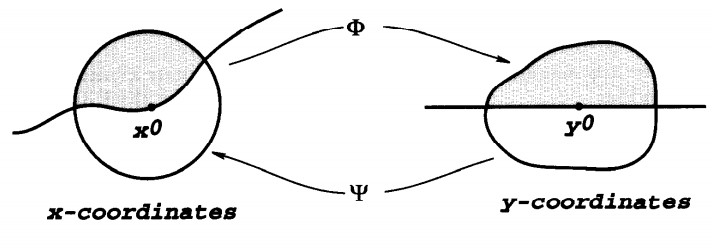
\includegraphics[scale=.5]{flatb}
\caption{Immagine da \cite[cap.8]{Evans}}
\end{figure}
\begin{remark}
Notiamo che $\Phi$ preserva l'eventuale analiticità della superficie $\Gamma^*$.
\end{remark}

Questa trasformazione ci fa capire come sia possibile scegliere di considerare  ``privilegiata''. Da qui in poi essa prenderà il nome di ``tempo'' e la indicheremo con la lettera $t$. Per essere più precisi rinominiamo le variabili nel modo seguente:
\begin{align*}
t & \leftarrow x_n \\
x & \leftarrow (x_1,\ldots , x_{n-1})
\end{align*}
Inoltre, introduciamo un po' di notazione che tornerà utile più avanti:
\begin{itemize}
\item chiamiamo $\Gamma_0 = \{t=0\}$.
\item indichiamo le derivate nel modo seguente: $D^\alpha_x D^j_t u$.
\end{itemize}
Concludiamo quindi che grazie alla trasformazione $\Phi$ otteniamo il nuovo problema:
\begin{equation}\label{gamma0prob}
\begin{cases}
F(x,t, D^\alpha_x D^j_t u)=0 & |\alpha | +j \leq k\\
D^j_t u (x,0)= \phi_j(x) & \text{per }j<k 
\end{cases}
\end{equation}
dove $u^*=u(\Phi)$.

\noindent\rule[0.5ex]{\linewidth}{0.2pt}

\begin{definition}
$\Gamma^*$ (o $\Gamma_0$) è non caratteristica se l'equazione su $\Gamma_0$ può essere riscritta in \textbf{forma normale} rispetto a $t$, ovvero se il problema \eqref{gamma0prob} può essere riscritto così:
\begin{equation*}
\begin{cases}
D_{t}^k u = G(x,t, D^\alpha_x D^j_t u) & |\alpha |+ j \leq k, \, j<k \\
D_t^ju = \phi_j & \text{ su } \Gamma_0, \, j<k
\end{cases} \\
\end{equation*}
\end{definition}

Per rendere più concreta questa definizione spesso si cercano delle condizioni sufficienti, ed eventualmente anche necessarie, perché l'equazione possa essere riscritta in forma normale, come abbiamo fatto noi nel paragrafo \ref{supcar} per i casi più semplici e come è stato fatto in \cite{Evans} e in \cite{Folland}.
Vediamo quindi di cosa si tratta, distinguendo i vari casi e ipotizzando di esserci già messi nella situazione \eqref{gamma0prob}:
\begin{itemize}
\item lineare e quasi-lineare: si richiede che $a_{(0,\ldots ,0,k)} \neq 0$ su $\Gamma_0$;
\item non lineare: si richiede la validità ipotesi teorema della funzione implicita (noto anche come teorema del Dini) su $F$, ovvero $D_{(D^k_t u)} F \neq 0$ su $\Gamma_0$.
\end{itemize}

\begin{remark}
Sempre rimanendo nell'ipotesi che la superficie sia $\Gamma_0$, a partire da queste considerazioni è facile vedere come la nuova definizione di superficie non caratteristica sia coerente con le definizioni del paragrafo \ref{supcar}.
\end{remark}

Ricordiamo, infine, che la nozione di superficie caratteristica ci deve garantire la possibilità di calcolare tutte le derivate parziali della soluzione sulla superficie. Per questa ragione l'impostazione di questa costruzione si ispira, in parte, a \cite[cap.3]{Evans}, dove è presente la dimostrazione di questa proprietà in due passi:
\begin{enumerate}
\item prima si ragiona ipotizzando di essere su $\Gamma_0$;
\item grazie alla trasformazione $\Phi$ si ottiene la proprietà per una generica $\Gamma^*$.
\end{enumerate}


\newpage
\section{Serie di potenze}
Dando per nota la teoria delle funzioni olomorfe, e di conseguenza anche la teoria base delle funzioni analitiche (reali), in questo paragrafo vogliamo scoprire, o conoscere meglio, solamente degli strumenti molto specifici che ci permetteranno di dimostrare il TCK.

Cominciamo con lo studiare uno sviluppo in serie di potenze di una funzione di cui non dobbiamo dimenticarci.
\begin{definition}
Funzione maggiorante: $$\mathcal{M}_{Cr}(x)=\frac{Cr}{r-(x_1+\ldots +x_n)}$$
\end{definition}
Utilizzando il teorema multinomiale, dimostriamo che la questa funzione può essere sviluppata in serie di potenze per $|x|<r/n$, ricavandone l'espressione dei coefficienti $c_\alpha$:
\begin{align*}
\mathcal{M}_{Cr}(x) &= \frac{Cr}{r-(x_1+\ldots +x_n)} = C \sum\limits_{j=0}^\infty \left(\frac{x_1+\ldots +x_n}{r}\right)^j  \\
&= C \sum\limits_{j=0}^\infty \frac{1}{r^j} \sum\limits_\alpha  \binom{|\alpha |}{\alpha } x^\alpha = \sum\limits_\alpha 
\underbrace{C \frac{|\alpha |!}{\alpha ! \, r^{|\alpha |}}}_{c_\alpha} \, x^\alpha .
\end{align*}

A partire da questo risultato, vogliamo enunciare due teoremi, che costituiscono la spina dorsale del cosiddetto metodo dei maggioranti, ideato per la prima volta da Cauchy, e che permettono di giustificare la terminologia introdotta poco fa.

\begin{theorem}[utilità del maggiorante]\label{teomagg}
\hpth{
g_\alpha \geq |f_\alpha|\\
\sum g_\alpha x^\alpha \text{ ha raggio di conv. } R
}{
\sum f_\alpha x^\alpha \text{ha raggio almeno } R
}
\end{theorem}


\begin{theorem}[costruzione del maggiorante]
\hpth{
\sum f_\alpha x^\alpha \text{ ha raggio } R
}{
\exists \, r<R, \, C>0 : \, |f_\alpha | \leq C \frac{|\alpha |!}{\alpha ! \, r^{|\alpha |}}
}
\end{theorem}

\begin{proof}
E' sufficiente notare che prendendo $C \geq |f_\alpha r^{|\alpha |}|$ si ha come conseguenza immediata che
$$|f_\alpha | \leq C \frac{1}{r^{|\alpha |}} \leq C \frac{|\alpha |!}{\alpha ! \, r^{|\alpha |}}.$$
\end{proof}

Nel caso in cui valgano le ipotesi del teorema \ref{teomagg} scriveremo:  $\sum g_\alpha x^\alpha \gg \sum f_\alpha x^\alpha$.

\begin{remark}
Gli stessi teoremi continuano a valere nel caso dei numeri complessi.
\end{remark}

Concludiamo il paragrafo e il capitolo con qualche proprietà per la manipolazione di serie di potenze. 
Prima di tutto occupiamoci dell'operazione di composizione.
\begin{theorem}
\hpthml{
y: \mathbb{R}^n \rightarrow \mathbb{R}^m \text{ tale che } y(x) = \sum y_\alpha (x-x_0)^\alpha \text{ in intorno di } x_0\\
g: \mathbb{R}^m \rightarrow \mathbb{R}^d \text{ tale che } g(y) = \sum g_\beta (y-y_0)^\beta \text{ in intorno di } y_0=y(x_0)\\
f = g \circ y
}{ 
\exists \; f_\gamma = P_\gamma (g_\beta, \, y_\alpha \text{ con } \alpha_i \leq \gamma_i) \text{ insieme di coeff. tali che } \\
- \; P_\gamma \text{ polinomi a coeff. non negativi }\\
-  \; f (x) = \sum f_\gamma (x-x_0)^\gamma
}
\end{theorem}
\begin{remark}
La forma dei polinomi $P_\gamma$ non dipende da $g$ e $y$.
\end{remark}
\begin{proof}
è facile convincersi di questo scrivendo esplicitamente la composizione delle due serie, specialmente per quanto riguarda il fatto che il coefficiente $f_\gamma$ dipenda solo dagli $y_\alpha$ tali che $\alpha_i \leq \gamma_i$.
\end{proof}

Ponendoci per semplicità nell'origine e recuperando la notazione $(x,t)$ del paragrafo precedente, enunciamo una semplice riscrittura di questo teorema.
\begin{theorem}[composizione]\label{composizione}
\hpthml{
y: \mathbb{R}^n \rightarrow \mathbb{R}^m \text{ tale che } y(x,t) = \sum y_{\alpha j} \; x^\alpha t^j \text{ in intorno dell'origine}\\
g: \mathbb{R}^m \rightarrow \mathbb{R}^d \text{ tale che } g(y) = \sum g_\beta \; y^\beta \text{ in intorno dell'origine }\\
f = g \circ y
}{
\exists \; f_{\gamma k} = P_{\gamma k} (g_\beta, \, y_{\alpha j} \text{ con } j \leq i) \text{ insieme di coeff. tali che } \\
- \; P_{\gamma k} \text{ polinomi a coeff. non negativi }\\
-  \; f (x,t) = \sum f_{\gamma k} \; x^\gamma t^k \label{seriepol} \numberthis
}
\end{theorem}

Un altro modo per ottenere una serie della tipologia in \eqref{seriepol} è sfruttare una derivazione rispetto a una qualsiasi variabile $x_i$. Vediamolo con il seguente teorema.
\begin{theorem}[derivazione]\label{derivata}
\hpth{
y: \mathbb{R}^d \rightarrow \mathbb{R}^m \text{ tale che } y(x,t) = \sum y_{\alpha j} \; x^\alpha t^j \text{ in intorno dell'origine}\\
}{
f=D_{x_i}y \text{ è una serie di potenze come in \eqref{seriepol} in intorno dell'origine}
}
\end{theorem}
\begin{proof} derivando termine a termine otteniamo
$$ D_{x_i} \sum y_{\alpha j} \; x^\alpha t^j = \sum  \underbrace{(\alpha_j+1) \, y_{(\alpha+e_i)j}}_{f_{\alpha j}} \; x^\alpha t^j. \; \footnotemark$$ \footnotetext{$e_i$ multi-indice vale 1 in corrispondenza della sua componente i-esima e 0 altrimenti}
E' immediato verificare le altre proprietà di $f_{\alpha j}$.
\end{proof}

Infine, siamo interessati a vedere cosa succede quando moltiplichiamo due serie come in \eqref{seriepol}, ottenute con uno dei metodi (teoremi \ref{composizione} e \ref{derivata}), a partire da una stessa serie $y$.
\begin{theorem}
\hpth{
f^1, f^2 \text{ serie costruite con uno dei due metodi a partire da una stessa } y
}{
f = f^1 f^2 \text{ è una serie di potenze come in \eqref{seriepol} in intorno dell'origine }
}
\end{theorem}

\begin{remark}
E' ammissibile anche il caso misto, in cui $f^1$ è ottenuta con una composizione e $f^2$ con una derivazione, e sarà proprio quello che utilizzeremo.
\end{remark}

\begin{proof} possiamo ricavare l'espressione dei coefficienti di $f$:
$$f_{\gamma k} = \sum_{\substack{\omega+\theta=\gamma \\ l+h=k}} f^1_{\omega l}\;  f^2_{\theta h}\, .$$
Di conseguenza $f_{\gamma k}$ sarà sicuramente un polinomio a coefficienti non negativi, poiché questa proprietà viene preservata da somme e prodotti. Inoltre, notando che $l,\, h \leq k$, si può mostrare che ogni singolo polinomio $f_{\gamma k}$ eredita la proprietà degli $f^1_{\omega l}$ e $f^2_{\theta h}$, vale a dire che esso dipende solo dagli $y_{\alpha j}$ dove $j \leq k$.
\end{proof}


%\chapter{The Cauchy-Kowalevski Theorem} \label{invariant}

Now that we have developed all the necessary tools, let us assume we have any Cauchy problem. As we showed in section \ref{pb}, it can be rewritten in the form:
$$
\begin{cases}
F(x,t, D^\alpha_x D^j_t u)=0 & |\alpha | +j \leq k\\
D^j_t u (x,0)= \phi_j(x) & \text{for }j<k 
\end{cases}
$$
Consequently, we will only deal with this last case, where the conditions are assigned on $\Gamma_0=\{ t=0 \}$.

The fundamental assumption of this chapter is that the data ($F$ and $\phi_j$) are analytic in a neighborhood of the origin, a property that we will use to show the existence of a unique \textbf{analytic solution}, still in a neighborhood of the origin.

However, to guarantee existence, we are forced to make some assumptions about the structure of the equation. 
Considering what has been said in the previous chapter, especially regarding theorem \ref{teoescar}, intuition suggests that it might be a good idea to consider the surface $\Gamma_0$ to be \textbf{non-characteristic}. 
This property allows us to rewrite the equation again in an even simpler form, namely:
\begin{equation}\label{pbnorm}
\begin{cases}
D_{t}^k u = G(x,t, D^\alpha_x D^j_t u) & |\alpha |+ j \leq k, \, j<k \\ 
D_t^ju = \phi_j & \text{ on } \Gamma_0, \, j<k
\end{cases} \\ 
\end{equation}
This idea will allow us to prove the CKT.
\begin{namedtheorem}[Cauchy-Kowalevski Theorem]
\hpth{
\text{Problem \eqref{pbnorm}}\\
G, \, \phi_j \text{ analytic in a neighborhood of the origin}
}
{\exists ! \; u \text{ analytic solution in a neighborhood of the origin}}
\end{namedtheorem}


After keeping as general a view as possible, we want to understand how to prove the result we have in mind. The approach we will follow will be "in reverse," progressively generalizing the results. Indeed, we will start from the least general case until we reach that of an equation in normal form, effectively following the chronological order of the results.


\newpage
\section{ODEs}

First, let us tackle a theorem very similar to the CKT, which deals with the case of a system of ODEs in normal form. 
We will start by stating the theorem.

\begin{theorem}\label{teoedo}
\hpth{
A \subseteq \mathbb{C}, \, B\subseteq \mathbb{C}^n \text{ open }\\
\Omega \subseteq A \text{ open connected}\\
f:A\times B\rightarrow\mathbb{C}^n \text{ holomorphic}\\
\text{Pb: }
\begin{cases}
y' = f(x,y) \quad \forall x \in \Omega \\ 
y(x_0)=y_0
\end{cases}\\
}
{
\text{locally, there exists a unique holomorphic solution}
}
\end{theorem}

\begin{remark}
This does not exclude the possibility of finding other non-analytic solutions.
\end{remark}

This result was the first application of the theory of holomorphic functions in combination with the method of majorants, which, as we already know, was proposed by Cauchy in the first half of the nineteenth century. 
We do not provide the full proof because it uses a different majorant from the one we introduced in section \ref{powerseries} (i.e., the one we will use to prove the CKT). 
In any case, it can be found in \cite{Delf}, and the structure of the reasoning is the same as that of theorem \ref{teoquasilin}.

Although we do not address the issue of existence in detail, it is worthwhile to discuss exhaustively the problem of \textbf{uniqueness} of analytic (or holomorphic) solutions. An analytic function is uniquely determined by all its derivatives at a point, which, in this case, are known due to the analyticity of the function $f$.
We completely conclude the discussion by also addressing the situation of a PDE: here too, assuming the data are analytic, it is possible to know all the partial derivatives of the function, thanks to the fact that the surface on which the conditions are assigned is assumed to be non-characteristic.

Since this result has been demonstrated by constructing a majorant for the solution $y$, it is possible to obtain an estimate of its radius of convergence by using theorem \ref{theomaj}.

\begin{theorem}
\hpthml{
\text{Assumptions of theorem \ref{teoedo}}\\
\exists \, \overline{B_a(x_0)}\subseteq A,\,\overline{B_b(y_0)} \subseteq B\\
M=\max_{B_a(x_0),\, B_b(y_0)}|f|
}{
\text{The solution has radius at least } \widetilde{r}= a\left[ 1-\exp\left( -\frac{b}{aM(n+1)}\right) \right] 
}
\end{theorem}

\begin{remark}
It is interesting to note what happens when $B=\mathbb{C}^n$.
\end{remark}


\newpage
\section{Quasi-linear PDEs}

Now it is time to address the cornerstone of the entire reasoning about PDEs, namely the theorem that shows the existence, and thus also the uniqueness, of an analytic solution to a quasi-linear system of PDEs in normal form.

\begin{theorem}\label{teoquasilin}
\hpth{
A_i, \, B \text{ analytic in a neighborhood of the origin }\\
\text{Pb: }
\begin{cases}
D_t \, y = \sum\limits_{i=1}^{n-1} A_i(x,y)D_{x_i}y+B(x,y) \; \\ 
y=0 \quad \text{ on } \Gamma_0
\end{cases}
\\
}{
\exists ! \; y(x,t): \mathbb{R}^n \rightarrow \mathbb{R}^m
\text{ analytic solution in a neighborhood of the origin}
}
\end{theorem}

\begin{remark}
This theorem can easily be modified by replacing analyticity with \textbf{holomorphy}, in order to obtain a statement similar to the case of ODEs, as the extension is immediate since no particular assumption distinguishes the real case from the complex one in the proof.
\end{remark}

\begin{proof}
First of all, let us denote by $a^i_{ml}$ the components of $A_i$ and $b_m$ those of $B$, while the coefficients of the series are respectively $(a^i_{ml})_\gamma$ and $(b_m)_\gamma$. Now let us proceed step by step.
\begin{enumerate}
\item Considering component by component, we assume $y_h = \sum c^h_{\alpha j} x^\alpha t^j$ with ${h=1,\ldots, m}$.
\item The Cauchy condition tells us that $c^h_{\alpha 0}=0$.
\item By inserting the series for $y,\, A_i,\, B$ into the equation and using theorems \ref{composition}, \ref{derivative} and \ref{product}, we obtain for each row $h$ the equation:
$$\sum\limits_{\alpha, \, j} (j+1)c^h_{\alpha (j+1)}\, x^\alpha t^j = \sum\limits_{\alpha,\, j} P_{\alpha j}\left((c^h_{\alpha l})_{l\leq j},(a^i_{ml})_\gamma, (b_m)_\gamma\right) \, x^\alpha t^j$$
where the polynomials $P_{\alpha j}$ are naturally non-negative coefficients.
\item Thanks to this operation, we derive a recursive formula for the coefficients:
$$ c^h_{\alpha (j+1)}= (j+1)^{-1} P_{\alpha j}\left((c^h_{\alpha l})_{l\leq j},(a^i_{ml})_\gamma, (b_m)_\gamma\right),$$
which allows us to conclude that $c^h_{\alpha j} = Q_{\alpha j}\left((a^i_{ml})_\gamma, (b_m)_\gamma\right)$ where $Q_{\alpha j}$ are always polynomials with non-negative coefficients, the form of which does not depend on $A_i$ and $B$. Thus, we can also say that it is always possible to construct a power series that satisfies the equation. We are left to understand whether it converges with a positive radius.
\newpage
\item Now suppose we have another problem with the same structure defined by the functions $\widetilde{A}_i $ and $\widetilde{B}$ and we know a local analytic solution $\widetilde{y}$. We want to show that $$\widetilde{A}_i \gg A_i, \, \widetilde{B} \gg B \implies \widetilde{y} \gg y.$$
Considering that for both problems the same considerations hold up to point 4 (the polynomials $Q_{\alpha j}$ are the same!), we can write the following chain of inequalities:
\begin{align*}
\left|c^h_{\alpha j}\right| &= \left|Q_{\alpha j}\left((a^i_{ml})_\gamma, (b_m)_\gamma\right)\right|\\
&\leq Q_{\alpha j}\left(\left|(a^i_{ml})_\gamma\right|, \left|(b_m)_\gamma\right|\right) 
& \text{non-negative coeff.}\\
&\leq Q_{\alpha j}\left((\widetilde{a}^i_{ml})_\gamma, (\widetilde{b}_m)_\gamma\right) = \widetilde{c}^h_{\alpha j}
& \widetilde{A}_i \gg A_i, \, \widetilde{B} \gg B
\end{align*}
\item The last step consists in choosing $\widetilde{A}_i, \, \widetilde{B}$, in such a way as to explicitly calculate $\widetilde{y}$ and show that it is analytic. Given our knowledge about the power series that come from theorem \ref{constmaj}, we know how to construct an upper bound for $A_i$ and $B$. Thus, we select two constants $C$ and $r$ such that 
$$\frac{Cr}{r-(x_1+\ldots +x_{n-1})-(y_1+\ldots +y_m)}=\mathcal{M}_{Cr}(x,y) \gg A_i(x,y),\, B(x,y)$$
and that satisfy the inequalities \eqref{r} and \eqref{C}. We then define the problem
\begin{equation*}
\begin{cases}
D_t \, \widetilde{y}_h = \mathcal{M}_{Cr} (x,y) \left[\sum\limits_{i,\, j} D_{x_j}\widetilde{y}_i+1 \right] \\ 
\widetilde{y_h}=0 \quad \text{ on } \Gamma_0
\end{cases}
\end{equation*}
where $h=1,\ldots, m$. At this point it is possible to show, using the method of characteristics for quasi-linear first-order equations (paragraph \ref{metodocar}), that it has the solution
\begin{equation}\label{maggiorante}
\widetilde{y}_h(x,t)=u(x_1+\cdots +x_{n-1},\,t) \quad \forall h
\end{equation}
where
\begin{equation}\label{sol}
u(s,t)=\frac{r-s-\sqrt{(r-s)^2-2tCrmn}}{mn},
\end{equation}
which is clearly analytic in a neighborhood of the origin. See \cite[cap.1]{Folland} for the complete unfolding of the calculation.
\item We conclude by observing an interesting fact: there is nothing specific that guarantees that the solution found continues to ensure the upper bound. In fact, it is important to verify that $\widetilde{y}$ satisfies the inequality $|(x,\widetilde{y}(x,t))|< r$ (so that $\mathcal{M}_{Cr}$ is indeed a power series). For more details, see proposition \ref{prop}.
\end{enumerate}
\end{proof}


\newpage
As in the case of the system of ODEs, if we utilize theorem \ref{theomaj}, we can estimate the radius of convergence by studying the radius of the dominating solution in \eqref{maggiorante}. 

\begin{theorem}\label{stimaraggio}
The solution of Theorem \ref{teoquasilin} converges with a radius of at least
$$\widetilde{r} = \dfrac{1}{n-1}\, \dfrac{r}{8Cmn} \text{ with } C \geq \frac{1}{2}$$
\end{theorem}
\begin{remark}
$n \geq 2$ for the system to be truly in partial derivatives. 
\end{remark}
\begin{remark}
It is interesting to focus on the behavior with respect to $r$, knowing that:
\begin{align}\label{r}
r <& \min \{ \textit{radii of convergence of the coefficients } a^i_{ml}, \, b_m\} \\ 
\label{C}
C \geq & \max \begin{Bmatrix}
\max\limits_{i,m,l,\alpha } \left| (a^i_{ml})_\alpha \, r^{|\alpha |}\right|\\
\max\limits_{m,\alpha} \left|(b_m)_\alpha \, r^{|\alpha |}\right|
\end{Bmatrix}
\end{align}
\end{remark}

\begin{proof}
Let us fix $r$ and $C$ as above, and furthermore assume that $C \geq 1/2$ (we can do this without any problem). 
Initially, we focus on the function in \eqref{sol}, which is analytic in a neighborhood of the origin, particularly in the set 
$$A = \left\{ (s,t) \in \mathbb{R}^2 : t<\frac{(r-s)^2}{2Crmn} \right\} .$$
That is, it can be expanded in a power series in $B_l(0)$ with $0<l<d=\text{dist}(0, \partial A)$.
\begin{center}
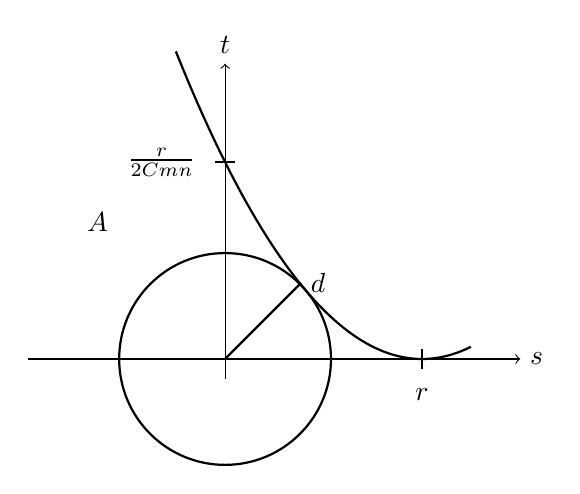
\begin{tikzpicture}[scale=2.5]
    % Draw the circle centered at (0,0) with radius 0.538
    \draw[thick,black] (0,0) circle[radius=0.538];
    
    % Draw the parabola y = (1-x)^2
    \draw[thick,black,domain=-0.25:1.25,samples=100] 
        plot ({\x}, {(1-\x)^2});
    
    \node[black,anchor=south west] at (-0.75, 0.60) {$A$};
    
    % Draw the axes
    \draw[->] (-1,0) -- (1.5,0) node[right] {$s$};
    \draw[->] (0,-0.1) -- (0,1.5) node[above] {$t$};
    
    % Draw the segment from (0,0) to (sqrt{0.538/2}, sqrt{0.538/2})
    \draw[thick,black] (0,0) -- (sqrt{0.538/1.9},sqrt{0.538/1.9});
    \node at (sqrt{0.538/1.9},sqrt{0.538/1.9}) [right] {$d$};
    
    % Draw the ticks
    \draw[thick] (1, 0.05) -- (1, -0.05); % Tick at (1, 0)
    \node at (1, -0.1) [below] {$r$};    % Label for (1, 0)
    
    \draw[thick] (-0.05, 1) -- (0.05, 1); % Tick at (0, 1)
    \node at (-0.1, 1) [left] {$\frac{r}{2Cmn}$}; % Label for (0, 1)
    
\end{tikzpicture}
\end{center}
Choosing $l_1 = (n-1)\,\widetilde{r}$, it can be shown that, for $C>1/8$, we indeed have that $l_1<d$. The goal would therefore be to verify that $$\sqrt{l_1^2-s^2} < \frac{(r-s)^2}{2Crmn}$$ for every $|s|<l_1$, but this is implied by 
\begin{equation} \label{l1}
l_1 < \frac{(r-l_1)^2}{2Crmn}\; ,
\end{equation}
an inequality that holds true if and only if $C > 1/(4mn) \leq 1/8$.

Now, we will generalize this for the function $\widetilde{y}_h$ in \ref{maggiorante} with $h$ fixed. It is analytic in the region 
$$A = \left\{ (x,t) \in \mathbb{R}^n : t<\frac{(r-(x_1+\ldots +x_{n-1}))^2}{2Crmn} \right\} .$$
The structure of the problem remains the same, so, naturally, the definition of $d$ remains unchanged. The only aspect we need to take care of is that, in this situation, it will be necessary to choose $l_2 =\widetilde{r}$. 
Thus, we want to show that $$\mathcal{L}=\sqrt{l_2^2-(x_1^2+\ldots +x_{n-1}^2)} < \frac{(r-(x_1+\ldots +x_{n-1}))^2}{2Crmn}=\mathcal{R}$$
when $|x|=|(x_1,\ldots ,x_{n-1})|< l_2$. But this is implied by the inequality \ref{l1}, which we know to be true. We will prove it in two steps.
\begin{itemize}
\item It holds that $\mathcal{L}^2< l_2^2 \leq l_1^2$ for $|x|< l_2$.
\item It holds that $$\left(\frac{(r-l_1)^2}{2Crmn}\right)^2 \leq \min \left\{ \mathcal{R}^2 : |x|\leq l_2 \right\}< \mathcal{R}^2 \, \text{ for } \, |x|< l_2.$$
This is shown knowing that $$\max \left\{ x_1+\ldots +x_{n-1} : |x|\leq l_2\right\}= (n-1)\frac{l_2}{\sqrt{n-1}}\leq l_1$$ and showing that $r-(x_1+\ldots +x_{n-1})>0$ for $|x|\leq l_2$ with the triangle inequality.
\qedhere
\end{itemize}
\end{proof}

\noindent\rule[0.5ex]{\linewidth}{0.2pt}

A careful reader will surely wonder about the reason behind choosing a constant $C\geq 1/2$. Well, this issue arises from what was left open in the proof of Theorem \ref{teoquasilin}, namely the fact that the solution $\widetilde{y}$ is indeed dominating only if $|(x,\widetilde{y}(x,t))|< r$. This property is precisely guaranteed in a ball of radius $\widetilde{r}$. Let us see this with a proposition that, in addition to clarifying, completes the logical framework of the proofs.
\begin{namedtheorem}[Proposition]\label{prop}
The domination of $\widetilde{y}$ holds in $B_{\widetilde{r}}(0)$, i.e.
$$|(x,t)|<\widetilde{r} \implies |(x,\widetilde{y}(x,t))|=x_1^2 + \ldots + x_{n-1}^2 + m \, u^2(x_1 + \ldots + x_{n-1},t) < r^2$$
\end{namedtheorem}
\begin{proof}
For simplicity, we demonstrate that $$|(s,t)|< l=(n-1)\,\widetilde{r} \implies s^2 + m \, u^2(s,t) < r^2.$$ The generalization is trivial if we take inspiration from the proof of Theorem \ref{stimaraggio}. 
\newpage
Considering that $|t|,|s|<l<r$ and that $s^2+t^2<l^2=r/(8Cmn)$, we write the following chain of inequalities.
\begin{align*}
& s^2 + m \left[ \frac{r-s-\sqrt{(r-s)^2-2tCrmn}}{mn} \right]^2\\ 
&\leq s^2 + \frac{1}{mn^2} \left[ (r-s)^2 + |(r-s)^2-2tCrmn| \right] 
&\begin{system}
\left|s\right| < r \Rightarrow r-s > 0\\
 \sqrt{(r-s)^2 - 2t Cr mn} > 0 
\end{system}\\
&\leq s^2 + \frac{2}{mn^2} (r-s)^2 + \frac{2|t|Crmn}{mn^2} \\ 
&\leq l^2 + \frac{2}{mn^2} \left( r^2 + l^2 + 2rl \right) + \frac{2lCrmn}{mn^2} 
&\begin{system}
\left|s\right| < l \Rightarrow (r-s)^2 < (r+l)^2\\
\left|t\right| < l
\end{system}\\
&= \left( \frac{r}{8Cmn} \right)^2 + \frac{2r^2}{mn^2} \left[ 1+\frac{1}{(8Cmn)^2} + \frac{1}{4Cmn} + \frac{1}{8} \right] \\ 
&< r^2 \underbrace{\frac{2}{mn^2} \left[ \frac{r}{8} + \frac{1}{(8C)^2 mn^2} + \frac{r}{(8Cmn)} + \frac{r}{4Cmn} + \frac{1}{8} \right]}_{<1} < r^2 \\ 
\end{align*}
In particular, the last statement holds because
\begin{align*}
n \geq 2 \Rightarrow \frac{2}{mn^2} \left(\ldots\right) 
&\leq \frac{1}{2} \left(\frac{9}{8} + \frac{2}{(8C)^2} + \frac{1}{8C}\right) \\ 
& \leq \frac{3}{16} \left(3 + \frac{1}{C}\right) < 1 & \Leftarrow C \geq \frac{1}{2} 
\end{align*}
\end{proof}



\newpage
\section{EDP in Normal Form}
Now we will utilize the results from the previous section to generalize that result to the case of an equation in normal form. To do this, it is sufficient to state and prove the following theorem.
\begin{theorem}\label{teonorm}
The following two problems are equivalent
\begin{align*}
\text{non-linear: }&
\begin{cases}
D_{t}^k u = G(x,t, D^\alpha_x D^j_t u) & |\alpha |+ j \leq k, \, j<k \\ 
D_t^ju = \phi_j & \text{ on } \Gamma_0, \, j<k 
\end{cases} \\ 
\text{quasi-linear: }&
\begin{cases}
D_t \, y = \sum\limits_{i=1}^{n-1} A_i(x,y)D_{x_i}y+B(x,y) \; \\ 
y=0 \quad \text{ on } \Gamma_0 
\end{cases}
\end{align*}
\end{theorem}

\begin{proof}
The reasoning is divided into three steps:
\begin{enumerate}
\item We construct the system such that $y_{\alpha j}= D^\alpha_x D^j_t u$. \\ 
Then, the matrices $A_i$ and $B$ can be obtained from the expressions
\begin{align*}
D_t y_{\alpha j} =& y_{\alpha (j+1)} & |\alpha| + j < k \\ 
D_t y_{\alpha j} =& D_{x_l} y_{(\alpha-e_l)(j+1)} & |\alpha| + j = k, \; j < k \\ 
D_t y_{0k} =& D_tG + \sum_{|\alpha|+j < k} D_{y_{\alpha j}}G y_{\alpha (j+1)} \\ 
& + \sum_{|\alpha|+j = k, \; j < k} D_{y_{\alpha j}} G D_{x_l} y_{(\alpha-e_l)(j+1)}
\end{align*}
where $l(\alpha)=\min\{ l:\alpha_l\neq 0 \}$, and the Cauchy data will be
\begin{align*}
y_{\alpha j}(x, 0) = & D_x^{\alpha} \phi_j(x) & j < k \\ 
y_{0k}(x, 0) = & G\left( x, 0, D_x^{\alpha} \phi_j(x) \right) & \lvert \alpha \rvert + j \leq k, \; j < k 
\end{align*}
\item We remove the conditions $\phi$, redefining $y(x,t)\leftarrow y(x,t)-\phi (x)$.
\item We eliminate the dependence on $t$, adding the variable $y^0=t$, together with the equation $D_t y^0=1$ and the data $y^0(x,0)=0$.
\end{enumerate}
We conclude by stating that, obviously, if $u$ is a solution of the problem in normal form, the $y_{\alpha j}$ will be solutions of the newly constructed problem. However, to demonstrate that $y_{(0,\ldots,0)}$ (solution of the latter) is also a solution of the problem in normal form, various calculations are necessary, which can be found in detail in \cite[cap.1]{Folland}.
\end{proof}

\begin{remark}
There are three aspects, which also emerge from the proof, that are worth briefly reflecting upon:
\begin{itemize}
\item Bringing together the considerations made at the beginning of the chapter and the theorems \ref{teoquasilin} and \ref{teonorm}, the CKT follows immediately;
\item The estimate of the radius of convergence continues to hold;
\item This equivalence theorem can be readily generalized to the case of a system in normal form.
\end{itemize}
\end{remark}

%

%\include{chapters/6alternatives}
%\chapter{Conseguenze}
\section{Teorema di Holmgren}

\section{Altre applicazioni}
teorema inutile nella pratica che però ha ispirato ricerche e scoperte future cruciali e utili (come accadde per i grafi di eulero)

applicazioni:
\begin{itemize}
\item fisica matematica (cosa succcede nella realtà quando si hanno soluzioni analitiche locali?)
\item teorema di holmgren
\item teorema di cartan-kahler (pag 137) utile in geometria differenziale (suggerisce Tao), economic theory (microeconomia, ekeland e chiappori, 1999) per l'eistenza locale di una funzione utilità concava (e quindi con un massimo) ricavata da un sistema di pdes che neccessita di dati analitici (visto come un sistema differenziale esterno)
\end{itemize}

I. Ekeland

Cartan Kahler

4 (with Chiappori), "Aggregation and market demand: an exterior differential calculus viewpoint", Econometrica, 67 (1999), p. 1435-1458

This paper solves a basic problem in economic theory, which had remained open for thirty years, namely the characterization of market demand functions. The method of proof consists of reducing the problem to a system of nonlinear PDEs, for which convex solutions are sought. This is rewritten as an exterior differential system, and is solved by the Cartan-Kähler theorem, together with some algebraic manipulations to achieve convexity. The introduction of exterior differential calculus proved to be a breakthrough, and was the starting point of a long collaboration with P.A. Chiappori. We realized that the mathematical structure we had discovered in this problem was to be found also in one of the major problems of econometrics: given a group (a household, for instance), can one characterize and identify the preferences of each member if one observes only the collective demand ?. I am happy to say that this research program is now concluded, with the publication of two major papers [14] and [25] and a100-pages survey [28] which will probably turn into a book.

14: (with P.A. Chiappori) "The microeconomics of group behaviour: general characterization". Journal of Economic Theory, september 2006 , volume 130 (p.1 – 26)

25: (with P.A. Chiappori) "The microeconomics of group behaviour: Identification". Econometrica, 2005, 44 pages

28: (with P.A. Chiappori). "The mathematics and economics of aggregation". Foundations and Trends in Economic Theory, 2009

% BIBLIOGRAFIA
% PER FARLA FUNZIONARE: eseguire latex-bibtex-latex-latex
\addcontentsline{toc}{chapter}{Bibliography}
\nocite{*} % Inserire nella bibliografia anche le fonti non citate esplicitamente nel testo
\bibliographystyle{alpha} % We choose the "plain" reference style
\bibliography{bibliography} % Entries are in the refs.bib file

\end{document}